\chapter{Hardware Design}

\section{Providing Test Data}
In order for the driver to stress the DUT, the verification system must perform at a much higher frequency than the expected frequency of the DUT.
Assuming the DUT is to run at 300MHz, to fully explore the effect of overclocking, the testbench must be able to run at double the frequency.
This gives an ambitious target frequency of 600MHz.
Assuming a data width of 32-bit, the target data transfer rate is then estimated to be 19.2Gbps.
With this rough estimate, we can start considering different design options.

\subsection{HPS-FPGA Bridge}
As the testing is to be controlled by the HPS, the HPS-FPGA bridge will be the immediate bottleneck if the test data is to flow from HPS to FPGA.
While the HPS can easily generate test data with a piece of software, there is a large amount of overhead as data crosses from one architecture to another.
This overhead exists in the form of both decreased bandwidth and increased delay.
Thus, it is not be sensible for the HPS to send out data during runtime.

\subsection{Off-chip DDR SDRAM}
Another thought may be to first populate the off-chip DDR SDRAM on the FPGA side, then feed that data to the DUT during test.
This is already much faster than passing the data directly from HPS.
The 1GB, 32-bit wide DDR3 on the FPGA side is rated at 400MHz.
With double rate transfer, this gives a maximum transfer rate of 25.6Gbps.

Although using the off-chip RAM may theoretically achieve the targets, it still has its disadvantages.
Firstly, the process of filling up the memory takes time.
Thus, the testing would be broken up into bursts, with time in between for checking results and filling in new data.
The complexity of the SDRAM interface also requires an SDRAM controller to be used to manage SDRAM refresh cycles, address multiplexing and interface timing.
These all add up to significant access latency.
While it could be overcome with burst and piplined accesses, it would further complicate the SDRAM controller.
A controller is provided by Intel~\cite{Altera3}, but it would consume a non-negligible amount of the limited FPGA resources while adding unnecessary complexities to the design.
Customising or building a new SDRAM controller to fit this project is possible, but needlessly time-consuming.

\subsection{On-chip Memory}
The on-chip memory is much faster and simpler to use.
In comparison, this memory is implemented on the FPGA itself, and thus needs no external connections for accesses.
It has higher throughput and lower latency than the SDRAM.
The memory transactions can also be piplined, giving one transaction per clock cycle.
With an on-chip FIFO accessed in dual-port mode, the write operations at one end and the read operations at the other end can happen simultaneously.
This feature is useful as tests are prepared and fed into the DUT, or when test results are collected and fed to the monitor.

On-chip memory is not without its drawbacks.
It is volatile like SDRAM and very limited in capacity.
SDRAMs can have store about 1GB, while on-chip memory could only hold a few MB~\cite{Altera2}.
Volatility is not exactly of concern in this project, but its small capacity means not much test data can be held before it needs more fed in.

\subsection{Distributed RAM / Registers}
On-chip memory has a minimum latency of 1 clock cycle as the R/W access gets processed.
If a even faster memory is desired, we can use LUTs or registers to store them.
This option would eliminate the latency but takes up much more FPGA resources.
The capacity is even more limited as LUTs are usually used for logic.
There will be a significant amount of data generated during testing, and the testbench should be as lightweight as possible to allow flexibility in the DUTs.
As such, distributed RAM will not be used in this project for data transfer.
Registers will still be used as they are essential for many other purposes.

\subsection{Real Time Data Generation}
As seen from the analysis, the best design option here should be able to exploit the benefits of on-chip memory, and circumvent the drawback of buffering testing data generated from the HPS.
Generating testing data at runtime, on the FPGA will be such a method.
As arithmetic operators have a vast set of valid inputs, it is necessary to have cost-effective test generation.

A good choice here is to use random testing.
With relatively low effort, random testing can provide significant coverage and discover relatively subtle errors~\cite{Duran1}.
The main drawback of random testing is the possible lack of coverage for corner cases, for which the usual solution is to provide handwritten tests to complement it.
However, as the main goal of this testbench is gauging the performance of the module, and not necessarily verifying the correctness of the module, having uncovered testing holes is acceptable during stress testing.
As the project progress, special tests could be written and run separately with a relaxed timing restriction to cover the holes.
It should be noted that certain corner cases may represent critical paths in the design.
To combat this, the testbench provides the option to run handwritten inputs alongside random tests.

\section{Randomiser}

LFSRs are a reliable way of generating pseudorandom numbers quickly with low cost~\cite{Hazwani1}.
Fulfilling the design requirements, they will thus form the starting point of data generation.
While it is possible for data generated to be invalid as inputs to the DUT, this should not be the case for most arithmetic units.
Even if this is the case, they can be dealt by the filter in the driver.
On the flip side, LFSRs go through every single possible value except for one before repeating itself in a loop, so it is more efficient than a purely random data set.
The one impossible value can be covered manually, and knowing that there is an impossible value from the randomiser can be turned into a design advantage later on when we make the driver.

Following this approach, the software would only need to configure the generation at the beginning, and test data no longer needs to pass through the HPS-FPGA bridge.
Thus, the testbench can provide fast and constant data to stress the DUT.

\subsection{LFSR Configurations}

While LFSRs are simple hardware modules, there are still a few design options we should explore before implementing them.
To compare, we can examine an 8-bit LFSR with taps on bit [7,5,4,3].

In a Fibonacci LFSR, the taps are pulled and fed into a cascade of XOR gates.
The output of the final XOR gate is then the lowest bit of the next random number.
The higher bits are obtained by one left bitwise shift.

\begin{figure}[H]
  \centering
  \begin{tikzpicture}
  [
    x=1em, y=1em,
    start chain = going left,
    node distance = 0em,
    reg/.style =
      {draw, minimum width=2em, minimum height=2em,outer sep=0pt, on chain},
    every join/.style={-, thick}
  ]
  \node [reg] at (0, 0) (1) {\texttt{0}};
  \node [reg] (2) {};
  \node [reg] (3) {};
  \node [reg] (4) {\texttt{3}};
  \node [reg] (5) {\texttt{4}};
  \node [reg] (6) {\texttt{5}};
  \node [reg] (7) {};
  \node [reg] (8) {\texttt{7}};

  \node [xor gate US,draw] at (-2.5, 2) (a) {};
  \node [xor gate US,draw] at (-5.5, 3) (b) {};
  \node [xor gate US,draw] at (-8.5, 4) (c) {};

  \draw (b.output) to[-|-] (a.input 1);
  \draw (c.output) to[-|-] (b.input 1);
  \draw (8.north)       |- (c.input 1);

  \draw (4.north)  |- (a.input 2);
  \draw (5.north)  |- (b.input 2);
  \draw (6.north)  |- (c.input 2);

  \draw [->, >=stealth] (a.output) -- (2, 2) |- (1.east);

\end{tikzpicture}
  \caption{Fibonacci Configuration}
  \label{FibLFSR}
\end{figure}

In a Galois LFSR, the new bits in the taps are obtained by a XOR operation between the lowest bit and the bit on the left of each tap.
The highest bit is simply the previous lowest bit, and all other bits are obtained by one right bitwise shift.

\begin{figure}[H]
  \centering
  \begin{tikzpicture}
  [
    x=1em, y=1em,
    start chain = going left,
    node distance = 0em,
    reg/.style =
      {draw, minimum width=2em, minimum height=2em, outer sep=0pt, on chain},
    spa/.style =
      {minimum width=3em, minimum height=2em, outer sep=0pt, on chain},
    every join/.style={-, thick}
  ]
  \node [reg] at (0, 0) (1) {\texttt{0}};
  \node [reg] (2) {};
  \node [reg] (3) {};
  \node [reg] (4) {\texttt{3}};
  \node [spa] ()  {};
  \node [reg] (5) {\texttt{4}};
  \node [spa] ()  {};
  \node [reg] (6) {\texttt{5}};
  \node [spa] ()  {};
  \node [reg] (7) {};
  \node [reg] (8) {\texttt{7}};

  \node [xor gate US,draw] at  (-8.4, 0) (a) {};
  \node [xor gate US,draw] at (-13.4, 0) (b) {};
  \node [xor gate US,draw] at (-18.4, 0) (c) {};

  \draw [->, >=stealth] (1.east) -| (2, -2) -- (-25,-2) |- (8.west);

  \draw (a.input 1-|5.east) -- (a.input 1);
  \draw (b.input 1-|6.east) -- (b.input 1);
  \draw (c.input 1-|7.east) -- (c.input 1);

  \draw  (-9.7,-2) |- (a.input 2);
  \draw (-14.7,-2) |- (b.input 2);
  \draw (-19.7,-2) |- (c.input 2);

  \draw (a.output) -- (4.west);
  \draw (b.output) -- (5.west);
  \draw (c.output) -- (6.west);

\end{tikzpicture}
  \caption{Galois Configuration}
  \label{GalLFSR}
\end{figure}

Other LFSR configurations such as Xorshift~\cite{Marsaglia1} exists, but they are mostly designed and optimised as pieces of software, thus being less appropriate for this design.

By examining the two configurations, we can see that Fibonacci LFSRs have to XOR multiple bits together through a cascade of 2 input XOR gates, or a single XOR gate with multiple inputs.
On the other hand, Galois LFSRs have multiple XOR gates working independently.
On an FPGA, the cascade of gates is usually implemented with a LUT, so while limiting LUT input to 2 might have some minor improvements, this increased delay of the Fibonacci configuration should not be obvious.

In terms of implementation, Fibonnaci LFSRs are slightly easier to code if width configurability is desired.
However, building a configurable Galois LFSR is only slightly more complex.

As such, we need to take a step back and examine the overall structure of the randomiser to help us make this decision.

\subsection{Randomiser Structure}

A horizontally structured randomiser uses all bits in the LFSR as output.

\begin{figure}[H]
  \centering
  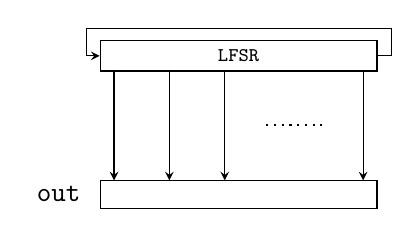
\begin{tikzpicture}
  [
    x=1em, y=1em
  ]
  \node at (-1.5, 0) {\texttt{out}};
  \node [draw,minimum height=1em, minimum width=10em] at (5, 0) (o) {};
  \node [draw,minimum height=1em, minimum width=10em] at (5, 5) (1) {\scriptsize \texttt{LFSR}};
  \draw [->, >=stealth] (1.east) -| ++(0.5, 1) -- ++(-11, 0) |- (1.west);
  \foreach \pos [count=\idx] in {0.5, 2.5, 4.5, 9.5}{
    \draw [->, >=stealth] (\pos, 4.5) -- (\pos, 0.5);
  }
  \draw [dotted, thick] (6, 2.5) -- (8, 2.5);

\end{tikzpicture}
  \caption{Horizontal Structure}
  \label{HoriLFSR}
\end{figure}

A vertically structured randomiser uses multiple LFSRs, and combines one bit from each LFSR for its output.

\begin{figure}[H]
  \centering
  \begin{tikzpicture}
  [
    x=1em, y=1em
  ]
  \node at (-1.5, 0) {\texttt{out}};
  \node [draw,minimum height=1em, minimum width=10em] at (5, 0) (o) {};
  \foreach \pos [count=\idx] in {0.5, 2.5, 4.5, 9.5}{
    \node [draw,minimum height=1em, minimum width=5em, rotate around={90:(0, 0)}] at (\pos, 5) (\idx) {\scriptsize \texttt{LFSR}};
    \draw [->, >=stealth] (\idx.west) -- (\idx.west|-o.north);
    \draw [->, >=stealth] ($(\idx.west)-(0, 0.5)$) -| (\pos-1,8) -| (\idx.east);
  }

  \draw [dotted, thick] (6, 5) -- (7.5, 5);

\end{tikzpicture}
  \caption{Vertical Structure}
  \label{VertLFSR}
\end{figure}

The horizontal option is easy to construct, but changing the width of the output value requires writing another wider LFSR since the tap positions would change.
The vertical options is much more scalable as more or less LFSR can be instantiated depending on the required output width.
As the widths of individual LFSRs are not related to the width of the output, a series cheap, 2-tap LFSRs can be used for it, making the earlier point of additional delay for Fibonacci LFSRs a non-issue.

However, the vertical structure is not without downsides.
Each LFSR needs a unique seed for its initialisation, making increasing the width not completely automatic unless we also build something that generates these seeds.
More importantly, the structure reduces the test efficiency introduced by LFSRs.
A single LFSR will go through every non-zero value before repeating itself, the vertically arranged randomiser will have early repeats.

If we allow early repeats, then the horizontal structure can be easily scaled.
This is achieved by building a long LFSR and taking a trucated version of the output value when fewer bits are required for the tests.

As such, there is no real advantage of using the vertical structure.
With truncation providing the configurability in the horizontal structure, the slight advantage of the Fibonacci LFSRs in its ease to write is nullified.
Having the slight advantage in terms of speed for Galois LFSRs, they will be chosen as the randomiser design in this project.

\section{Driver}

The driver should have two main types operation when feeding data into the DUT.
One is the stress testing mode, where the driver tries to pushes a new piece of data into the DUT at every clock tick.
The alternative is a slow manual mode, where the driver reads from the HPS-FPGA bridge and changes its output to the DUT whenever a new test point is specified by the software.
The stress testing mode will expose the DUT to as much random test points as possible in the test duration.
The manual mode is used when the user has a special interest in a limited list of inputs.

\subsection{Stress Testing Mode}
The vanilla way of providing data to the DUT is to for the driver to simply instantiate the same number of randomisers as the number of inputs of the DUT.
Then the randomisers' outputs can be directly connected to the inputs of the DUT.

While this fast and cheap method fulfils most of the requirements of the testbench, it suffers from a few issues.
One, there is no user control for the test data.
If we consider the LFSR pseudo-random number sequence to be unpredictable, then the only thing the user can do will be forcing the LFSRs to initialise with same of different seeds and therefore the DUT will receive identical or different inputs.
However, this level of customisation mostly meaningless.

\subsection{Input Filtering}
To introduce some level of non-trivial user control in the test data without losing speed, a filtering system is included in the driver design.
The filtering system needs to be fast since this is still a stress test, yet it should provide as much utility as possible to the users.

A possible design here is to allow the user to specify a maximum and a minimum bound to the value of the input data.
Each output from the randomiser is compared to these values and either sent forward if they passed or replaced if they failed the comparisons.
If a higher level of control is desired, there can also be a list of invalid inputs within the bounds of validity.
However, the latency can get high if the list is long and the comparisons can get slow if the high or low bound is irregular in its binary form.
The replacement system can also get complex if the bounds are strict.

A better alternative to achieve this is a bit manipulation system.
The user can force individual bits in the data to be cleared or set.
This is less flexible than the first design, but with some tricks the user is still able to perform a great level of input control.
Having only odd or even test inputs will be trivial under this system.
To set maximums or minimums for the test data, the user can simply set or clear the higher bits.
Certainly this imposes a strong preference to arithmetic units with regular binary representations, but most interesting designs for high-radix arithmetic units, including the ones that spawned this project, use a radix that is a power of 2.
As such, the binary manipulation system will always be helpful for the user to filter out uninteresting test points or to focus in on more meaningful ones.

\subsection{Manual Input Mode}

As discussed in the randomiser section, random testing is surprisingly useful, but they do have their limits.
If the user has a list of inputs that will trigger key logic paths in their design, they should be able to investigate them under this framework.
This would serve as a good compliment to the random testing.
The manual input mode is designed for this scenario.
In this mode, the user first provides a list of numbers when configuring the test in software, and enable the manual input mode.
Then, the test software will read through this list and write them to a set of memory locations on the HPS-FPGA bridge.
A simple transfer protocol will be used for the driver to read these locations and then forward them to the DUT.
Due to the limitations of the bridge, the DUT cannot be fully saturated with these data.
As such, each manual test input will be repeatedly sent to the DUT before the next one becomes available.

\subsection{Synchronised Monitor Inputs}
In addition to controlling what gets sent to the DUT, the driver has the responsibility to ensure that the monitor receives the test output from the DUT and the test inputs from the driver at the same time.
After going through the filtering logic, the stream of test input will not only be sent to the DUT, but also sent to a shift register before reaching the monitor.
The shift register will provide the delay required for the DUT to finish its operations.
Since the number of cycle delay from input to output should be consistent and known by the user, the length of this delay can be configured before compiling the testbench.


\section{Monitor}

Another concern in the system design is of the different clock domains that must exist on the FPGA.
Since it is not sensible to require the reference design to run as fast as the DUT, there needs to be two clock domains in the system.
The initial idea is to have one domain surrounds the DUT and another that supports the rest of the control logic around the DUT.
These clock frequencies can be generated with PLLs, which are provided as IP Cores in the Quartus software~\cite{Altera4}.
A clock tree will distribute them to the individual modules.
Data crossing clock domains will be fed through FIFOs to prevent loss.

The proposed structure will have the bulk of the control logic running in a separate clock domain to the DUT.
Only an interface with FIFOs will be running in synchronicity with the DUT.
Therefore, the test controls can run at a slower frequency without bottlenecking the system, allowing the DUT to be stressed further.
The problem now is to ensure the monitor can handle the stream of DUT output coming in at a higher frequency that it is running at.
As the monitor needs to calculate the correct data before it can check if the DUT output is correct, it cannot keep up with the speed of the DUT.
This report consider three alternatives.

\subsection{Partial Monitors}
A lightweight idea is to implement a parity checker instead of a full model inside the monitors.
For example, to check an adder, the monitor can just check if the final bit with a LUT acting as a XOR gate.

Although this is reasonably fast, it cannot be extended once the DUT is faster than a parity calculation followed by a comparison.
More critically, it provides no additional information once the DUT fails, and it has a 50\% rate of ignoring an error.
If this is to be solved by increasing the number of bits checked, the problem returns back to its initial state.
Thus this method will not be experimented.

\subsection{Lazy Monitors}

\begin{figure}[H]
  \centering
  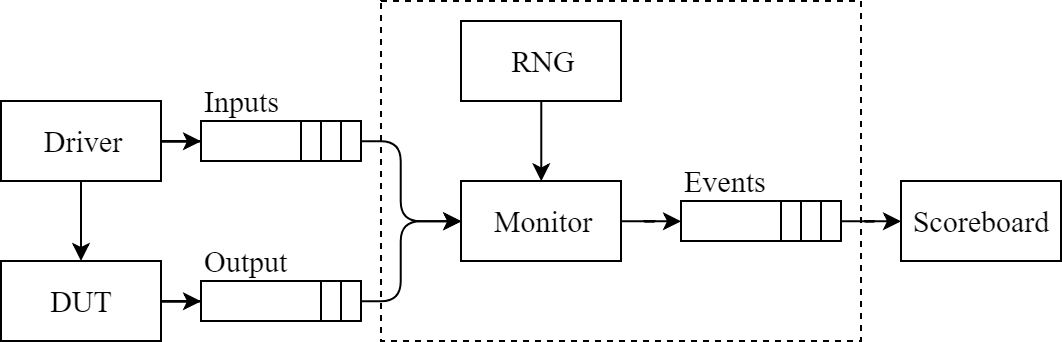
\includegraphics[width=12cm]{img/LazMon}
  \caption{Structure of a Lazy Monitor}
  \label{LazMon}
\end{figure}

An more scalable alternative is to have the monitor only check a selection of data sets.
For example, if the monitor is programmed to check every third test point, statistically it will make little difference to the final result.
In case the DUT is aware of this and only produce correct outputs on every third operation, this process can be randomised too.

This method can be extended if the DUT get fast simply by skipping more checks, and it has the full information when it detects an error.
However, this method needs the extra logic in the random controller, making the monitor slightly more complex than it probably should be.

\subsection{Parallel Monitors}

\textcolor{red}{These diagrams needs to be rebuilt to better reflect the idea. Or maybe even rebuilt with the simplified clock domain thing but that could also be done in the implementation chapter.}

\begin{figure}[H]
  \centering
  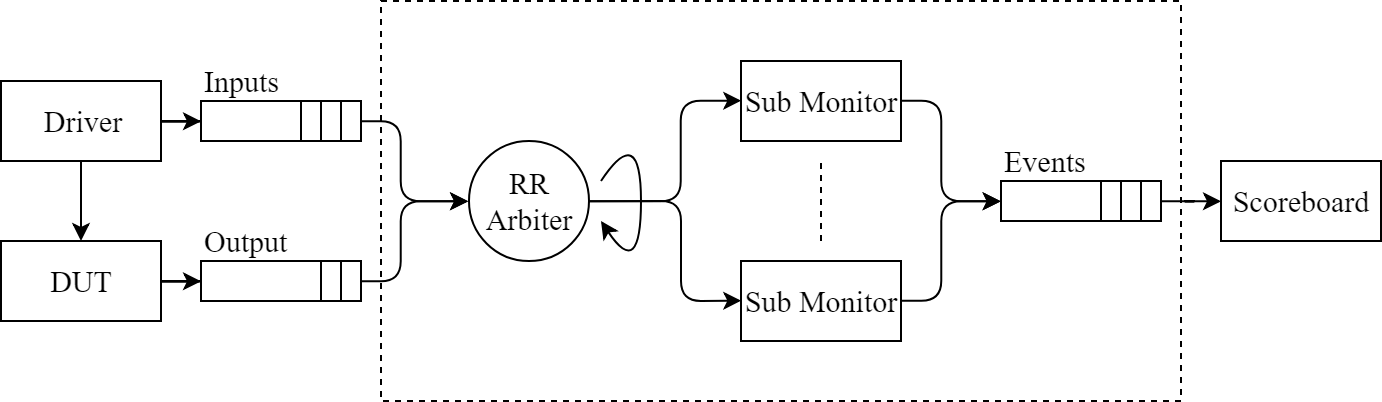
\includegraphics[width=15cm]{img/ParMon}
  \caption{Structure of a Parallel Monitor}
  \label{ParMon}
\end{figure}

As the test data is uniform, the monitor can be parallelised in to a number of sub-monitors.
The sub-monitors is connected to a distributor that is connected to three FIFOs.
The FIFOs are the inputs and the output of the DUT.
A round robin demultiplexer distributes the data to the sub-monitors equally.
The results from each sub-monitor are then sent to a single scoreboard.
To avoid potential hazards, the output from the sub-monitors will be buffered before processed by the scoreboard.

This does not have data dependency on a random controller, and it can fully guarantee the correctness of the DUT.
It is also scalable as more sub-monitors can be added it the DUT fills up its output buffer.
As a downside, this method takes up the most FPGA resources to implement as it scales.

Comparing across the three methods, the parallel monitors will be used for this project, as it offers the best functionalities.

\section{Simplified Clock Domains}
During the implementation of the parallel monitors, it is realised that picking the parallel structure has enabled a simpler way for us to realise the hardware design regarding clock domains.
So far, the assumption has been that during frequency testing, the testbench would hold on to a consistent frequency, while the frequency of the DUT is varied.
However, this causes unnecessary complications as the clock ticks of the two domains would shift in and out of phase during testing, which needs to be handled with extreme care since there is heavy data moving through the domains.

Looking back at the overall structure of the framework, the slowest block is the reference designs in the sub-monitors.
The priority of a reference design is to be functionally correct.
Since the operation it carries out can still be complex, it should have a relaxed timing requirement in order to avoid additional burdens on the designer.
This would hopefully make the reference relatively easy to produce and difficult to make mistakes on.
On the other hand, the rest of the testbench should be able to operate at the speed of the DUT, as they are relatively light in terms of the logical operations that they perform.
If a slow signal path arises in the system, it is also relatively harmless to sacrifice a few cycles in terms of latency to keep its maximum frequency high.

Therefore, instead of having a fast domain surrounding the DUT, the new design would have a slow domain surrounding the sub-monitor, while the rest of the testbench is clock at the same speed as the DUT.
The number of sub-monitors is a parametrised value, but it has to be an integer.
As such, the slow domain will always have a clock frequency that is a factor of the frequency of the rest of the testbench.
This way, they can stay in phase, which may have made the design of the monitor slightly more complicated, but vastly simplified the rest of the system.

\section{Scoreboard}
One of the simplification has to do with the connection from the monitor to the scoreboard.
Previously, there was no guarantee that the scoreboard would be synchronous with the sub-monitors producing the results of the tests.
This necessitated the event driven system, which would reduce the amount of traffic produced by the sub-monitors, and allows the scoreboard to keep track of more test data points that it normally could.
Now that the scoreboard runs on the fast clock, the monitor can simply produce one piece of information for each data point, and the scoreboard would be able to handle it.

Since the precision of results coming from the DUT is of interest to us, one possible use of this bandwidth is to pass on the precision of each test data to the scoreboard.
The scoreboard can then produce more detailed statistics from the test set.
Instead of only counting how many points are correct and how many are wrong, it will also be able to determine more interesting values such as the maximum and minimum precision of a test set.

These output values will be stored in registers which are exposed and can be read by the HPS.
If further statistics and insights are desired, it would be more sensible to perform these operations in the testing software.
